\chapter{Analysis and modeling}
\label{ch:analysis}
%\section{Intensity fluctuation and statistics}
%In this section, we look at the intensity fluctuation and their statistics in event 50, from fixed and moving sources respectively. Acoustic intensity data are derived from the complex demodulates of the match filter output as given by 
%%Eq.\ref{eq:intensity}. 


\section{ Intensity fluctuation and statistics}

%The propagation of acoustic signals is strongly related to the ocean's physical attributes with various time scales and frequencies, such as surface waves, internal waves, tides, currents. Given the condition in SW06 experiment  ( acoustic signal transmission interval = 4sec, acoustic listening window = 3hr), we concentrated ourselves to the variation caused by the internal wave activities. 
%
%Quantities will be used in the following sections are:
%
%(1) Integrated acoustic intensity  
%
%When the propagation and scattering conditions change in the water, the received acoustic intensity changes at the same time. We calculate the intensity of the signal arrivals integrated over a pulse
%length $\Delta\tau$ at a given depth $z$ as
%
%\begin{equation}\label{eq:intensity1}
%I(z,T)=\displaystyle\frac{1}{{\rho}c}\int\limits^{\tau+\Delta\tau}_{\tau}p^2(z,T,t)\,dt
%\end{equation}
%where $p$ is acoustic
%pressure,$\rho$ is water density, and $c$ is sound speed.
%And the total intensity integrated over the depth H is
%
%\begin{equation}\label{eq:intensity2}
%I(T)=\displaystyle\int\limits^H_0I(z,T)dz.
%\end{equation}
%The time integration at a single hydrophone is to show the attenuation and scattering through the medium, both horizontally and vertically, thus carries much information about the environment, in our case the internal wave packet. On the other hand, the depth integration over the entire water column gives the energy flux through a particular vertical slice, which is of great interests here because the change of this parameter shows how much energy is transported through the horizontal acoustic mechanisms like refraction and reflection, under the condition of constant attenuation and scattering. 
%We will examine the mean and standard deviations of the intensity at different stages during the passing of the internal wave packet. 
%
%(2) arrival time and pulse spread
%
%The passing of the internal waves also has an effect at the arrival time (sometimes called the "wander" in literature) and pulse spread. We define the arrival time as the arrival time of the centroid of the acoustic pulse.
%\begin{equation}\label{eq:arrival_time}
%t_c =\frac {\int\limits^{t_0}_{t_1}I(t)tdt}{\int\limits^{t_0}_{t_1}I(t)dt}
%\end{equation} 
%in which, $t_c$ is the arrival time, $t_0$ and $t_1$ are the beginning and the end time of a received pulse, $I(t)$ is the acoustic intensity. (All the time variables in the equation above $t_c$,$t_0$,$t_1$ are started from a common but arbitrary zero point, due to the lack of a absolute clock between the receiver and the transmitter. )
%There are other definitions of the "arrival time" in the literature, e.g. the leading edge arrival time and the peak arrival time. We choose the centroid definition due to its insensitivity to the swift changes of the arrival pulse structure, which are quite common in SW06 experiment.


%(3) correlation time and length

Based on the theory proposed in our previous work, the angle between
the ISW fronts and the acoustic track determines the mechanism of
the intensity fluctuations. Small angles provide horizontal
refraction and focusing while larger angles cause mode coupling.
Between these limits, there is an angular region for which the
propagation is adiabatic.  During internal wave Event 50, the ISW
fronts passed through the acoustic track at an angle of about $5^o$
providing the condition for horizontal refraction. Prior to the ISW
arrival, we observe stable adiabatic propagation in a stable water
column. Hence, a transition can indeed be observed between these two
mechanisms.

To show a focusing event, we consider two geotimes: (a) $T_{g1}$ when the
leading internal wave front had not reached the acoustic track and,
(b) $T_{g2}$ when the internal wave packet occupied most of the acoustic
track. We calculate the total intensity integrated over the depth H
as

\begin{equation}\label{eq:intensity}
I(T)=\displaystyle\int\limits^H_0I(z,T)dz
\end{equation}
where
$I(z,T)=\displaystyle\frac{1}{{\rho}c}\int\limits^{\tau+\Delta\tau}_{\tau}p^2(z,T,t)\,dt$
is the intensity of the signal arrivals integrated over a pulse
length $\Delta\tau$ at a given depth $z$, where $p$ is acoustic
pressure,$\rho$ is water density, and $c$ is sound speed. The
distribution of the ISWs in the horizontal plane can be assessed by
carefully examining the radar image and the depth distribution of
the temperature at three points (SW45, SW20, SW54) along the
acoustic track.

%\begin{figure}
 % \centering
 % 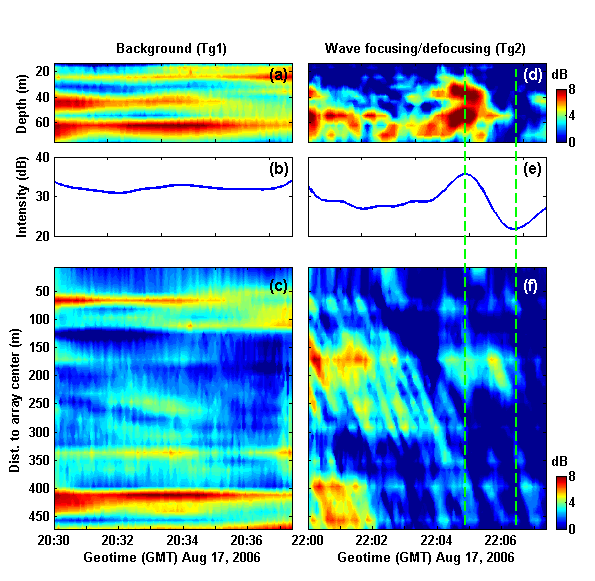
\includegraphics[width=0.75\textwidth]{jasa4.png}
 % \caption{Received acoustic intensity during a 440 sec (~ 7.33 mins) transmission period for two geotimes, $T_{g1}$ (from 20:30:00 to 20:37:20 GMT):  (a) depth distribution of total intensity per pulse I(z,T), (b) depth integrated intensity, I(T) for VLA, (c) total intensity I(x,T) for HLA; and $T_{g2}$ (22:00:00 to 22:07:20 GMT): (d) depth distribution of total intensity per pulse I(z,T), (e) depth integrated intensity, I(T) for VLA, (f) total intensity I(x,T) for HLA.}\label{fig:jasa4}
%\end{figure}
The temperature distribution starting at 20:30:00 GMT ($T_{g1}$) for the
transmission period (i.e. $\sim7.5$ minutes) at three different moorings
shows very little fluctuation along the acoustic track (see Fig.
2).This indicates that the ISW has not reached the acoustic track
during $T_{g1}$, as is also shown in the radar image. In Fig.\ref{fig:jasa4}(a) we
show a plot of I(z,T) for the VLA. It is shown that for a repeated
pulse of the same radiated intensity, only minor temporal intensity
variation exists.  In Fig.\ref{fig:jasa4}(b) we plot the depth integrated
intensity for all geotimes, I(T).  The very small fluctuations (~ 3
dB) at $T_{g1}$ indicate a quiescent condition without ISWs in the track.
This means that during this period of observation there is no
redistribution of sound energy in the horizontal plane, i.e. there
is no horizontal refraction. Small variations of the depth
distribution of the sound intensity correspond to the adiabatic
case. Fig.\ref{fig:jasa4}(c) shows the acoustic intensity on the HLA. There are
no apparent temporal intensity variations on the HLA during this
geotime.

I(z,T) for $T_{g2}$ is plotted in Fig.\ref{fig:jasa4}(d). Here we see increasing and
decreasing trends in sound intensity over the VLA, which are
synchronous in depth. The average intensity I(T) using Eq. (1) peaks
to ~ 35 dB around 22:04:30 to 22:05:00 GMT, and decreases to ~ 20 dB
around 22:06:37 GMT as shown in Fig.\ref{fig:jasa4}(e). This significant
fluctuation corresponds to redistribution of the acoustic energy in
the horizontal plane, which in the limit can be referred to as
focusing or defocusing events and is related to the position of the
source and/or receiver with respect to the internal wave crests. The
focusing and defocusing are also shown in Fig.\ref{fig:jasa3}(c) and Fig.\ref{fig:jasa3}(d). In
this case (i.e. $T_{g2}$), the receiver is between two adjacent maxima of
the thermocline displacement, and the high intensity fluctuations (~
15 dB peak to peak) are due to horizontal refraction effects similar
to those shown in previous studies.3 Temporal fluctuations correlate
with oscillations of the thermocline layer at the receiver (see Fig.
2) due to ISWs (period is ~ 7-8 min). The fluctuations in the
presence of internal waves (i.e. at $T_{g2}$) are about 15 dB, which are
much larger than those of $T_{g1}$ (~ 3 dB) with no internal wave in the
acoustic track. Although the total jump in the thermocline thickness
(i.e. from ~ 15 m to ~ 30 m) could make a difference in the
'absolute' value of the acoustic intensity, it does not play a
significant role in the temporal intensity fluctuation with periods
corresponding to the ISW.

As in the quiescent case shown above, Fig.\ref{fig:jasa4}(f) shows the acoustic
intensity on the HLA for the active period ($T_{g2}$). During the geotime
of about 7.33 minutes, we see the variation of the sound field at
the horizontal array. For the variation observed during the first 3
minutes, there are two large intensity maxima observed at the HLA.
These become weaker and disappear during the second half of the time
period (after 22:03 GMT). This behavior, in our opinion, is a
manifestation of horizontal redistribution of the sound intensity,
which we call focusing/defocusing phenomena. The sloped intensity
modulations correspond to the motion of an interference pattern
registered on the horizontal array, which can be a result from any
motion of the water layer (such as an ISW packet). The velocity of
this interference pattern is estimated as 1-1.5 m/s from the
acoustic data [shown as a slope in Fig. 4(f)]. This may not be
directly related to the velocity of the internal solitons (measured
from shipboard radar to be about 1 m/s). Further detailed modeling
is needed to understand the nature of these fluctuations and their
relationship to the slope of the lines shown in Fig. 4(f).


%\subsection{Fixed source}
%\subsection{Moving source}

\section{Acoustic signal coherence time and length}
The fluctuation of received acoustic signal can also be described with its coherence time and length using the lagged autocovariance function defined as


\begin{equation}\label{eq:autocov}
C_{i,t}=<I(t,z)I(t+\tau,z)>
\end{equation}

The autocovariance function is strongly dependent on the position of the internal wave front with respect to the acoustic path. 
\subsection{Fixed source}
Before IW, the autocovariance function (Fig
\subsection{Moving source}
\section{Behavior of horizontal ray beams}
\subsection{Horizontal Ray}
\subsection{Horizontal beamforming}
\subsection{Single mode propagation}
\subsection{Mode coupling}
\section{Horizontal Lloyd's mirror effect}
Introduction to optical Lloyd's mirror effect and acoustic equivalent.
\subsection{Two-dimensional case}
We start with 2D propagation case on the horizontal plane in an environment with an approaching wave front. This provides a concise picture of the relationship between the internal wave movement and the acoustic propagation. %Results from a more detailed horizontal-ray vertical-mode analysis and a Parabolic Equation simulation for a 3D environment are presented in later sections. 

We assume the high temperature front brought by internal waves is well mixed and is across the entire water column. This assumption effectively reduces the problem to a 2D case. Figure 3 shows the geometry of the simplified experimental setup on the horizontal plane. 
For a single frequency acoustic signal, the acoustic pressure at receiver can be written as
\begin{equation}\label{2D1}
p(r,t)=a_1e^{i(\omega t-kr_1}+a_2e^{i(\omega t-kr_2)}
\end{equation}
$r_1$ is the direct path between the source and receiver, and $r_2$ is the reflected (or refracted) ray path from the high temperature internal wave front in horizontal plane, hense a function of geotime $r_2=r_2(T)$ . Here, $a_1$  and $a_2$  are the amplitudes of acoustic wave along two paths. $\omega$  is the angular frequency,  $k$ is the acoustic wave number, and as usual,  $k=
\frac{\omega}{c}$,  where $c$ is the sound speed. 

The intensity of a sinusoidal acoustic signal $I=|p|^2$ is, 
\begin{equation}\label{2D2}
I(T)=a_1^2+a_2^2+2a_1a_2cos\{k[r_1-r_2(T)]\}
\end{equation}

Figure 4(a) shows a 7.5 min segment of the frequency dependent intensity pattern matching the LFM transmission in SW06 experiment. A 30min segment is plotted in Fig. 4(b) to show the long geotime trend that is the changing of the slope and the broadening of the stripes, as observed from experimental data in Fig. 2(d).

The period $ \Gamma$ and the slope of the beating interference patterns shown in Fig. 2(d) both increase as the internal wave front approaches the acoustic track. Although the slope only changes slightly during the 7.5min transmission time, it is a measurable quantity that can be calculated as follows. From Eq. ??, the angular frequency of the oscillating intensity as a function of  wave number $k$  is
\begin{equation}\label{2Dfreq1}
\Omega=\frac{d}{dt}k(r_1-r_2)
\end{equation}

If specular reflection assumption is used (i.e., the path shown by the dashed line in Fig. 3), $\Omega$ can be written in terms of the IW approaching speed $v$ , the source position $(0,y_s)$  and receiver position $(x_r ,0)$.
\begin{equation}\label{2Dfreq2}
\Omega(T)=2k\frac{(y_s-2vT)v}{\sqrt{x_r^2+(y_s-2vT)^2}}
\end{equation}

The period of the beating oscillations is simply $\Gamma(T)=2\pi/\Omega$ , and is a function of the geotime. As the IW front gets closer to the acoustic path, interference between the direct and reflected (or refracted) paths causes a beating pattern. Using the specular reflection assumption, we can write the period as 
\begin{equation}\label{2Dperiod}
T=\frac{\pi\sqrt{x_r^2+(y_s-2vT)^2}}{k(y_s-2vT)v}
\end{equation} 

The minima of the acoustic intensity  occurring at , from which the length difference of the two paths can be written as 
\begin{equation}\label{2D3}
r_1-r_2=(2n+1)\pi/k
\end{equation}
in which, the integer n represents the number of stripes. The acoustic frequency $f=kc/2\pi$  can be written as a function of geotime as 

\begin{equation}\label{2D4}
f=\frac{(2n+1)c}{2(r_1-r_2(T))}
\end{equation}

The slope $s=df/dt$  of the n-th stripe in the time-frequency spectrogram is
\begin{equation}\label{2D slope}
s=\frac{d}{dT}\left(\frac{(2n+1)c}{2(r_1-r_2(T))}\right)
\end{equation}

Using specular reflection assumption, 
\begin{equation}\label{2D slope2}
s=-c\cdot v(2n+1)\frac{(y_r+y_s-2vT)}{(r_1-r_2)^2r_2}
\end{equation}

The period and the slope in equations \ref{2Dperiod} and \ref{2D slope2} are plotted in Fig. ?? and ?? for $f=280Hz$, which is the frequency of the largest intensity in the received signal. To demonstrate the gradual increase of these variables, we show a 30-minute geotime segment prior to the IW arrival at the acoustic track. The IW reaches the receiver at 0 minute. At the -7 minute mark, the period $\Gamma=0.70min$  and the slope $s-50.83Hz/min$  respectively. These are in excellent agreement with the values in the experimental data at 21:37GMT, shown in Fig. ??. 

Next we discuss the intensity of a broadband LFM signal. The integrated acoustic intensity of a LFM signal can be written as:
\begin{equation}\label{2D broadband intensity}
I_{int}=(a_1^2+a_2^2)\Delta\omega+\frac{4a_1r_2c}{r_1-r_2}\left(sin\frac{\Delta k(r_1-r_2)}{2}\cdot cos(k_c(r_1-r_2))\right)
\end{equation}
\subsection{Three-dimensional case}

